\documentclass[11pt]{article}
\usepackage{geometry}
\geometry{margin=100pt}
\usepackage[utf8]{inputenc}
\usepackage{graphicx}
\usepackage{epstopdf}
\usepackage{titlesec}
\usepackage{biblatex}
\usepackage{float}
\usepackage{pdfpages}
\newcommand{\horrule}[1]{\rule{\linewidth}{#1}} 
\titleformat{\chapter}{\large\bfseries\centering}{}{0pt}{\huge}
\begin{document}
%opening

\title{
	\vspace{-30mm}
	{\LARGE Machnine Learning (PDEEC0049)\\ \Large Homework 3 }\\[80mm]
    {
\includegraphics[scale=0.1]{feup-logo}}\\[50mm]
}
\author{Shashank Gaur - UP201309443\\}
\date{\today}
\maketitle
\newpage
\section{Problem 1}

\section{Problem 2}

\section{Problem 3}
Following the calculation below, we ensure that the there is no difference in solutions obtained with two kernels provided in the problem

\begin{figure}[H]
	\centering
	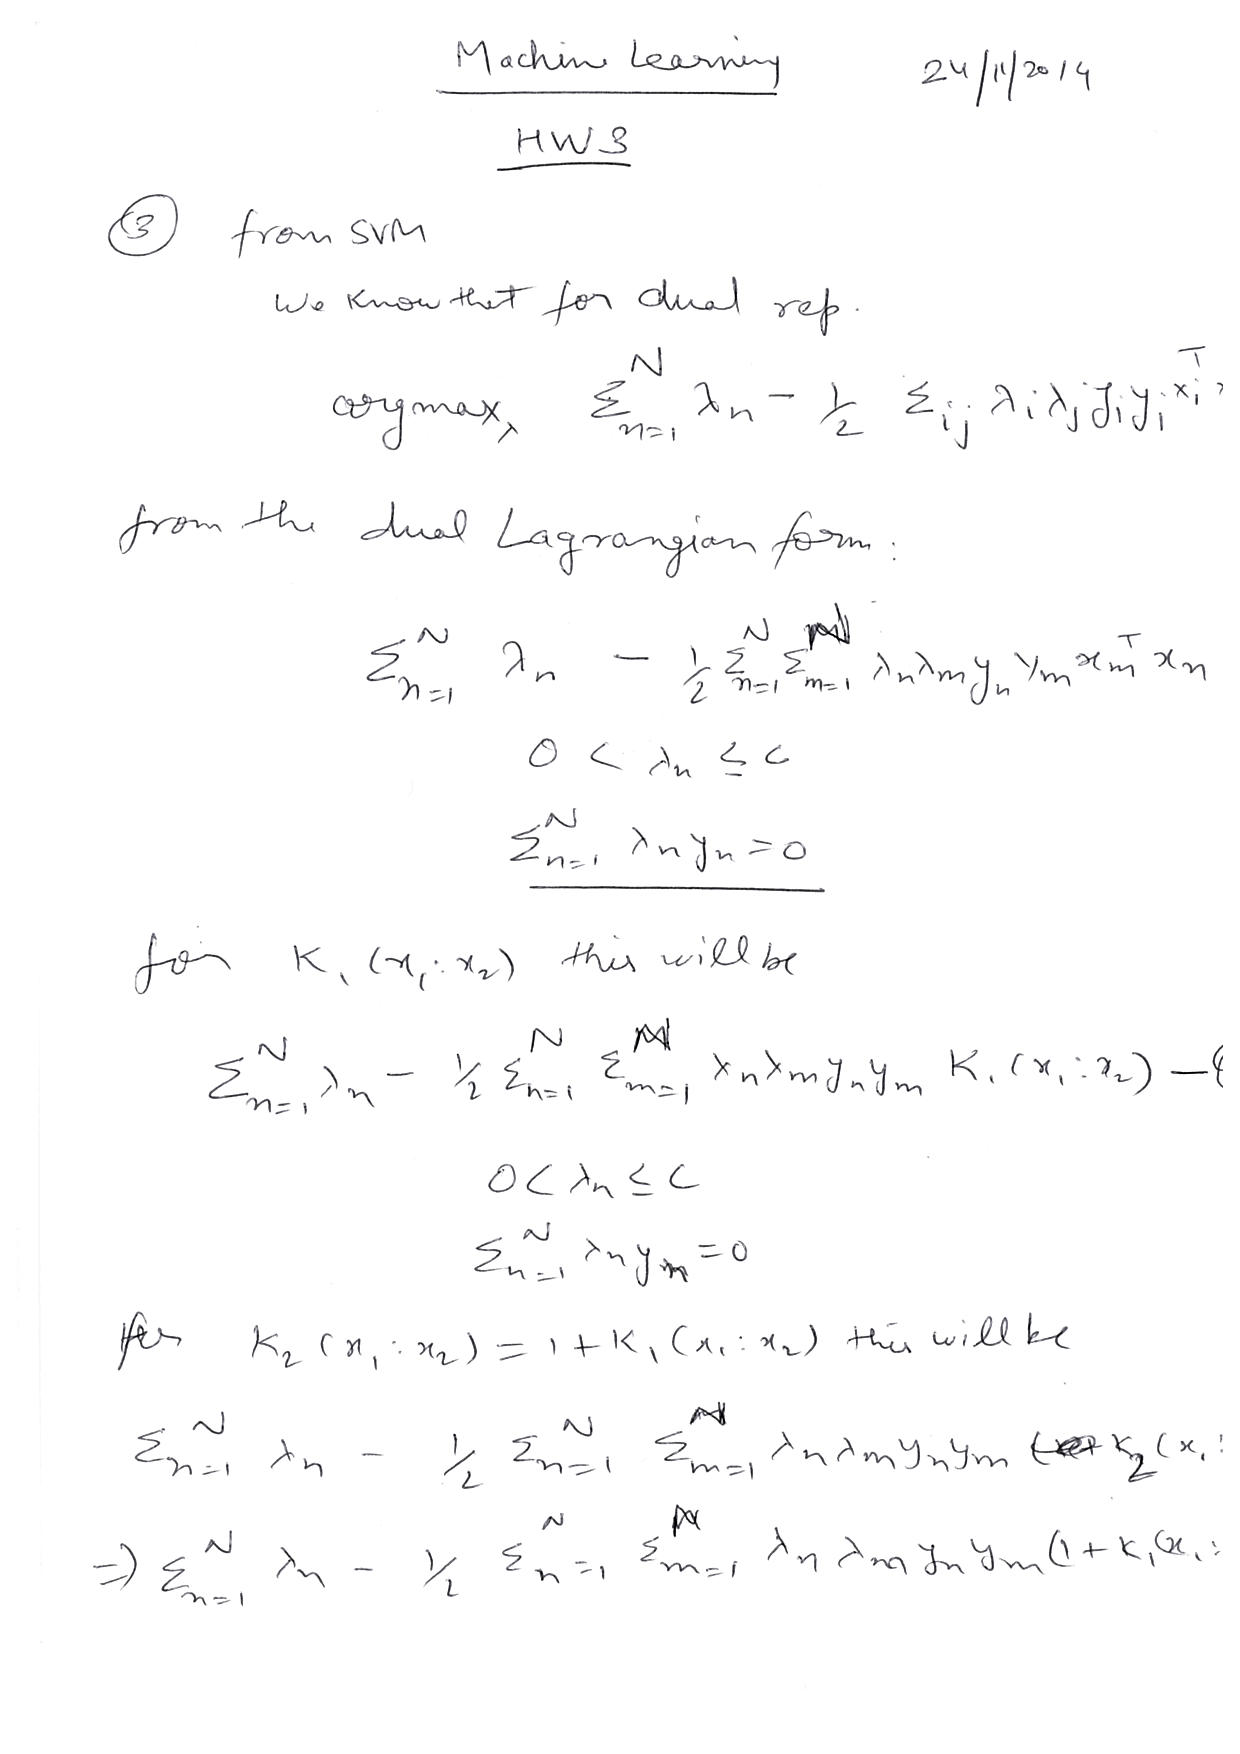
\includegraphics[page=1,scale=0.65]{scans}
\end{figure}

\begin{figure}[H]
	\centering
	\includegraphics[page=2,scale=0.65]{scans}
\end{figure}
.

\section{Problem 4}

Please run the testDAG to view the plots. 

\begin{figure}[H]
	\centering
	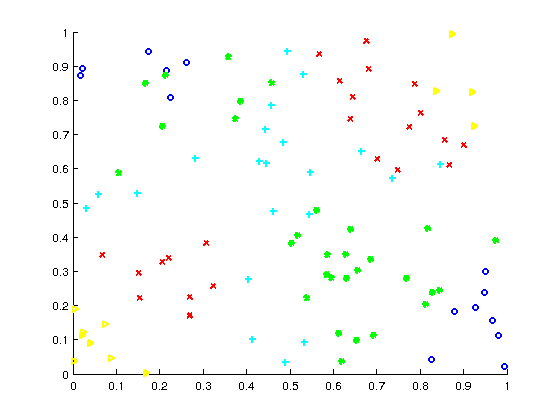
\includegraphics{1}
	\caption{training set}
\end{figure}
\begin{figure}[H]
	\centering
	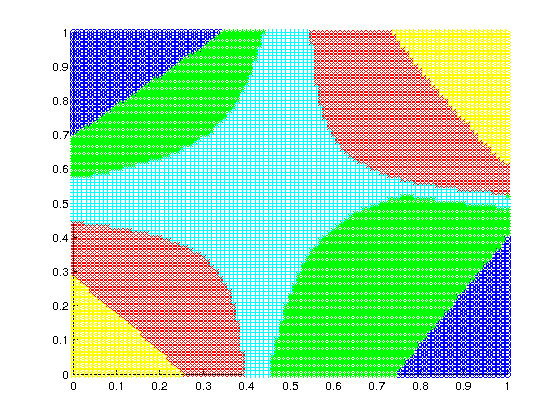
\includegraphics{2}
	\caption{From the libsvm function svmtrain}
\end{figure}
\begin{figure}[H]
	\centering
	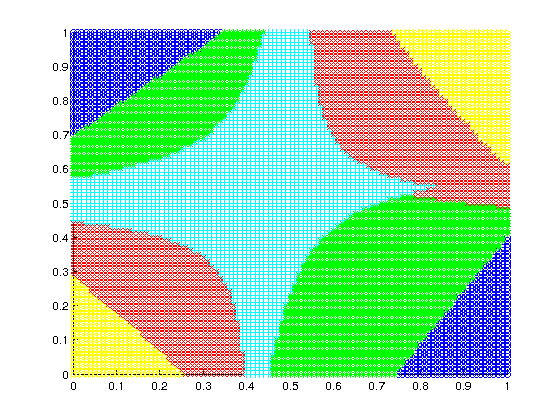
\includegraphics{3}
	\caption{from the SVM DAG function basicsvmtrain and basicsvmpredict}
\end{figure}

\end{document}